\model{Machine Instructions}

%TODO replace images from textbook (Copyrighted by Pearson -- fair use?)

\begin{multicols}{2}
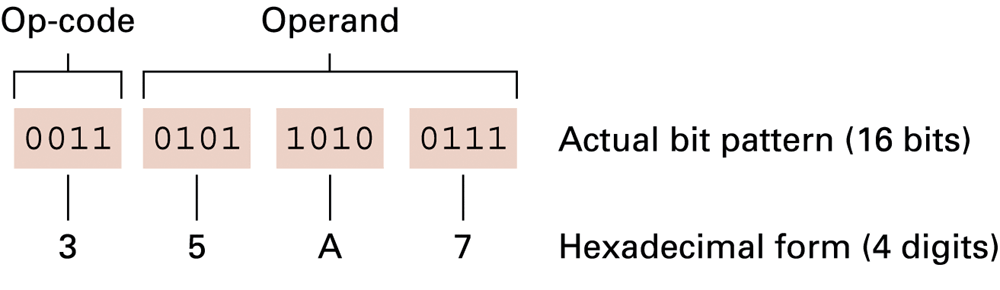
\includegraphics[width=\linewidth]{CSP/opcode1.png}

\columnbreak

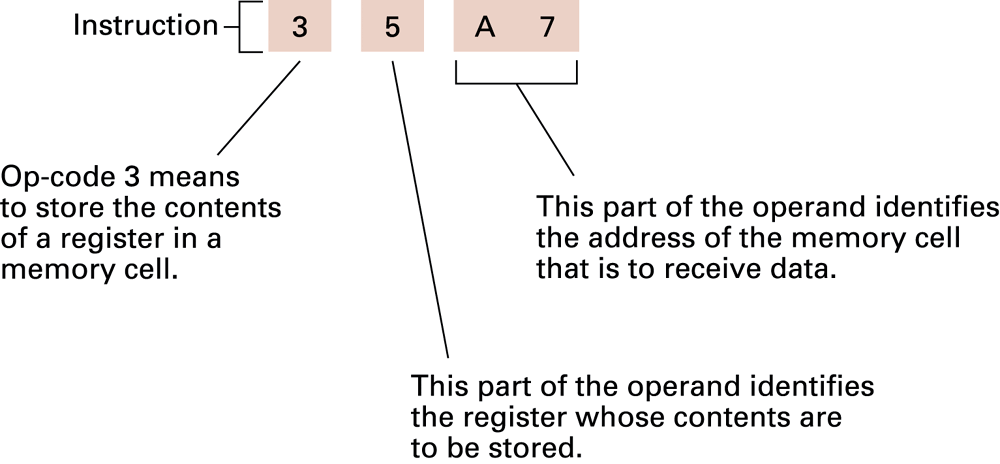
\includegraphics[width=\linewidth]{CSP/opcode2.png}
\end{multicols}


\quest{8 min}


\Q How many bits is the op-code? How many possible op-codes can the machine support?

\begin{answer}
With 4-bit op-codes, the machine can have at most 16 different op-codes.
\end{answer}


\Q The op-code for loading data from memory into a register is 1.
Write an instruction (in hex) for loading data from address 3D into register 4.

\begin{answer}
143D
\end{answer}


\Q Why is the instruction register in \ref{CSP/architecture} twice as large as the other registers?
How many memory cells are needed to store a single instruction?

\begin{answer}
Instructions are 16 bits, and memory cells are 8 bits; one instruction takes up two cells.
Note the instructions need to be large enough for their operand to represent a memory address.
\end{answer}
